\documentclass[]{beamer}
%\usepackage{babel}
\usepackage[latin9]{inputenc}
\usepackage{color,colortbl}
\usepackage{xcolor}
\usepackage{graphicx}
\usepackage{xmpmulti}
\definecolor{LRed}{rgb}{1,.8,.8}
\usepackage[T1]{fontenc}
\usepackage{tikz}
\usepackage{subscript}
\usepackage{subfigure}
\usepackage{beamerthemesplit} %// Activate for custom appearance
\usetheme{Berkeley} 
\usecolortheme{orchid}
\beamertemplatenavigationsymbolsempty

\makeatletter
\newcommand\insertlogoii{}
\newcommand\logoii[1]{\renewcommand\insertlogoii{#1}}
\setbeamertemplate{headline}
  {%
    \begin{beamercolorbox}[wd=\paperwidth]{frametitle}
      \ifx\beamer@sidebarside\beamer@lefttext%
      \else%
        \hfill%
      \fi%
      \ifdim\beamer@sidebarwidth>0pt%  
        \usebeamercolor[bg]{logo}%
        \vrule width\beamer@sidebarwidth height \beamer@headheight%
        \hskip-\beamer@sidebarwidth%
        \hbox to \beamer@sidebarwidth{\hss\vbox to
          \beamer@headheight{\vss\hbox{\color{fg}\insertlogo}\vss}\hss}%
        \hfill%
        \vrule width\beamer@sidebarwidth height \beamer@headheight%
        \hskip-\beamer@sidebarwidth%
        \hbox to \beamer@sidebarwidth{\hss\vbox to
          \beamer@headheight{\vss\hbox{\color{fg}\insertlogoii}\vss}\hss}%
      \else%
        \vrule width0pt height \beamer@headheight%  
      \fi%
    \end{beamercolorbox}
}
\makeatother
\renewcommand*{\thesubfigure}{}

%----PhYHeader------
% ***********************************************************

% ******************* PHYSICS HEADER ************************

% ***********************************************************

% \DeclareMathOperator{\Sample}{Sample}

\let\vaccent=\v % rename builtin command \v{} to \vaccent{}

\renewcommand{\v}[1]{\ensuremath{\mathbf{#1}}} % for vectors

\newcommand{\gv}[1]{\ensuremath{\mbox{\boldmath{#1}}}} 

\providecommand{\e}[1]{\ensuremath{\times 10^{#1}}} %Notaci�n cient�fica

\renewcommand{\o}[1]{\ensuremath{\mathbf{\widehat{#1}}}} %Comando para operadores

\newcommand{\f}[2]{\frac{#1}{#2}} %Establece el comando de fracciones

\newcommand{\uv}[1]{\ensuremath{\mathbf{\hat{#1}}}} % for unit vector

\newcommand{\abs}[1]{\left| #1 \right|} % for absolute value

\newcommand{\avg}[1]{\left< #1 \right>} % for average

\let\underdot=\d % rename builtin command \d{} to \underdot{}

\renewcommand{\d}[2]{\frac{d #2}{d #1}} % for derivatives

\newcommand{\dd}[2]{\frac{d^2 #2}{d #1^2}} % for double derivatives

\newcommand{\pd}[2]{\frac{\partial #2}{\partial #1}} % for partial derivatives

\newcommand{\pdd}[2]{\frac{\partial^2 #2}{\partial #1^2}} % for double partial derivatives

\newcommand{\pddc}[3]{\frac{\partial^2 #3}{\partial #1\partial #2}} % for double partial derivatives

\newcommand{\pdc}[3]{\left( \frac{\partial #1}{\partial #2}  \right)_{#3}} % for thermodynamic partial derivatives

\newcommand{\ket}[1]{\left| #1 \right>} % for Dirac bras

\newcommand{\bra}[1]{\left< #1 \right|} % for Dirac kets

\newcommand{\braket}[2]{\left< #1 \vphantom{#2} \right|

 \left. #2 \vphantom{#1} \right>} % for Dirac brackets

\newcommand{\matrixel}[3]{\left< #1 \vphantom{#2#3} \right|

 #2 \left| #3 \vphantom{#1#2} \right>} % for Dirac matrix elements

\newcommand{\grad}[1]{\v{\nabla} #1} % for gradient

\let\divsymb=\div % rename builtin command \div to \divsymb

\renewcommand{\div}[1]{\v{\nabla} \cdot #1} % for divergence

\newcommand{\curl}[1]{\v{\nabla} \times #1} % for curl

\newcommand{\Lap}[1]{\v{\nabla}^2  #1} % for Laplacian

\newcommand{\m}[1]{\textbf{ #1}} %for matrix

\newcommand{\mt}[1]{\m{#1}^\text{\tiny{$\intercal$}}} %for matrix transpose

\newcommand{\transpose}[1]{{#1}^\text{\tiny{$\intercal$}}} %for transpose

\newcommand{\mi}[1]{\m{#1}^\text{\tiny{-1}}} %for matrix inverse

\newcommand{\inverse}[1]{{#1}^\text{\tiny{-1}}} %for inverse

%\renewcommand{\labelenumi}{(\alph{enumi})} % Use letters for enumerate

\let\baraccent=\= % rename builtin command \= to \baraccent
\renewcommand{\=}[1]{\stackrel{#1}{=}} % for putting numbers above =

% ***********************************************************
% ********************** END HEADER *************************
% ***********************************************************

\title{Bayesian Hierarchical Modelling of Young Stellar Clusters}
\author{}

\logoii{
\includegraphics[width=1.2cm]{Logos/UNED-logo.jpg}}
\logo{
\includegraphics[width=2cm]{Logos/IPAG-logo.png}}
\institute{}
\date{\tiny{October 2017}}

\definecolor{olive}{rgb}{0.3, 0.3, .5}
\definecolor{beamer@blendedblue}{rgb}{0.3,0.3,0.8} % changed this
\setbeamercolor{structure}{fg=beamer@blendedblue}

\beamertemplatenavigationsymbolsempty 

\setbeamersize{sidebar width left=0pt}
\setbeamertemplate{footline}{}
\begin{document}

%%%%%%%%%%%%%%%%%%%%%%% INICIO %%%%%%%%%%%%%%%%%
\frame{
\frametitle{\hspace{2cm}Star clusters}
\begin{center}
%  \only<1>{\centering \includegraphics[height=\textheight]{Media/OrionAll.jpg}
%  \note{The majority of the stars are formed in groups} }
%  \only<2>{\centering \includegraphics[height=\textheight]{Media/OrionZoom.jpg}}
%  \only<3>{\centering \includegraphics[height=\textheight]{Media/OrionZoom2.jpg}
%  \note{Only one 10\% of the groups will survive bounded the first few hundred Myr}}
  \only<1>{\includegraphics[width=\textwidth]{Media/Pleiades.jpg}
  \note{Born together --> Homogeneous Properties\\
  Same space, distance, velocities, metallicites, age}}
  \only<2>{\includegraphics[width=0.7\textwidth]{Media/Pleiades-RADec.png}}
  \only<3>{\includegraphics[width=0.7\textwidth]{Media/Pleiades-pmRADec.png}}
  \only<4>{\includegraphics[width=0.8\textwidth]{Media/Pleiades-K_i_K.png}
  \note{More importantly their observables are also clustered. position in the sky, photometry, proper motions, parallax. 
- - Show images of clustered observables.
- Those observables are also be shared by millions of objects, including distant galaxies and other stars from our galaxy.  
- Entanglement
- Clusters typical sizes ranges from a few tens to a few thousands. 
- The problem is like finding a needle in a haystack.
- Even if we find them we are not certain.
- On top of that, we must remember that Astronomy is an observational science.
- We, like palaeontologist or archeologist, can not experiment!}}
\end{center}
}

%%%%%%%%%%%%%%%%%%%%%%%%%%%%%%%%%%%%%%%%%%%%%
\frame{
\frametitle{\hspace{2cm}Ideal vs. Reality}
\begin{columns}[T]
\begin{column}[T]{0.5\textwidth}
\begin{itemize}
\item Perfect tags
\item Properties of stars 
\begin{itemize}
\item 6D phase space (3D positions, 3D velocities)
\item luminosities
\item Metallicites
\item Ages
\item Temperatures and masses
\item Magnetic fields
\end{itemize}
\item All stars
\item Precision and accuracy
\end{itemize}
\end{column}
\begin{column}[T]{0.5\textwidth}
\begin{itemize}
\item Membership probabilities
\item Properties of some stars
\begin{itemize}
\item 2D positions, 2D proper motions, parallaxes, radial velocities
\item Apparent magnitudes
\item Metallicities
\item Masses (binaries)
\item ...
\end{itemize}
\item Global properties
\item Precision depends on distance/brigthness
\item Dependent on stellar models
\end{itemize}
\end{column}
\end{columns}
}

%%%%%%%%%%%%%%%%%%%%%%%%%%%%%%%%%%%%%%%%%%%%%%%
\frame{
\frametitle{\hspace{2cm}How things are done now?}
\begin{itemize}
\item BANYAN I {\footnotesize (Malo et al. 2013)}
\item UPMASK  {\footnotesize (Krone-Martins \& Motinho 2014)}
\item Sarro {\footnotesize (Sarro et al. 2014)}
\item BANYAN II {\footnotesize (Gagne et al. 2015)}
\item Sampedro  {\footnotesize (Sampedro and Alfaro 2016)}
\item LAceWing {\footnotesize (Riedel et al. 2017)}
\end{itemize}
}
%%%%%%%%%%%%%%%%%%%%%%%%%%%%%%%%%%%%%%%%%%%%%%%
\frame{
\frametitle{\hspace{2cm}Approaching the ideal}
%image of Sxitine chapel
\begin{columns}[T]
\begin{column}[T]{0.5\textwidth}
\only<1,2>{
\begin{itemize}
\item Global properties \note{In the form of probability distributions of: proper motions, positions and photometry}
\item Use as many objects as possible\note{observed and partially observed.}
\item Propagate uncertainties \note{with their correlations and propagate them to the global properties}
\end{itemize}
}
\end{column}
\begin{column}[T]{0.5\textwidth}
\only<2>{
\begin{itemize}
\item Parametric distributions\note{of the true positions, proper motions and photometric properties.}
\item Modelling missing values \note{as nuisance parameters, and marginalising them. (very simplistic assumptions) (Notice, I currently can not correct for the unobserved objects, except in some observables)}
\item Individual uncertainties \note{Each individual uncertainty is deconvolved (subtracted) in order to obtain the true value of the observable.}
\end{itemize}
\begin{enumerate}
\item Big data \note{Increase the size of the data set which the model is constructed}
\item All-Inclusive \note{All objects contribute to the global properties proportional to their membership probability.}
\end{enumerate}
}
\end{column}
\end{columns}
}
%%%%%%%%%%%%%%%%%%%%%%%%%%%%%%%%%%%%%%%%%%%%%
\frame{
\frametitle{\hspace{2cm}Strategy}
\begin{enumerate}
\item Chose a Cluster: the Pleiades.
\item Select a data set: DANCe DR2 (DDR2).
\item Create the methodology
\item Validate and get results
\item Compare to previous results 
\end{enumerate}
}
%%%%%%%%%%%%%%%%%%% PLEIADES %%%%%%%%%%%%%%%%%%%%%%%%%%%%
\frame{
\frametitle{\hspace{2cm}Pleiades History}

Sorry ... Next time!
%- members 
%- positions
%- distances
%- proper motions
%- luminosities
%- mass distribution
}
%%%%%%%%%%%%%%%%%%% DATA SET %%%%%%%%%%%%%%%%%%%%%%%%%%%%
\frame{
\frametitle{\hspace{2cm}DDR2(Bouy+2013)}
\centering
\only<1>{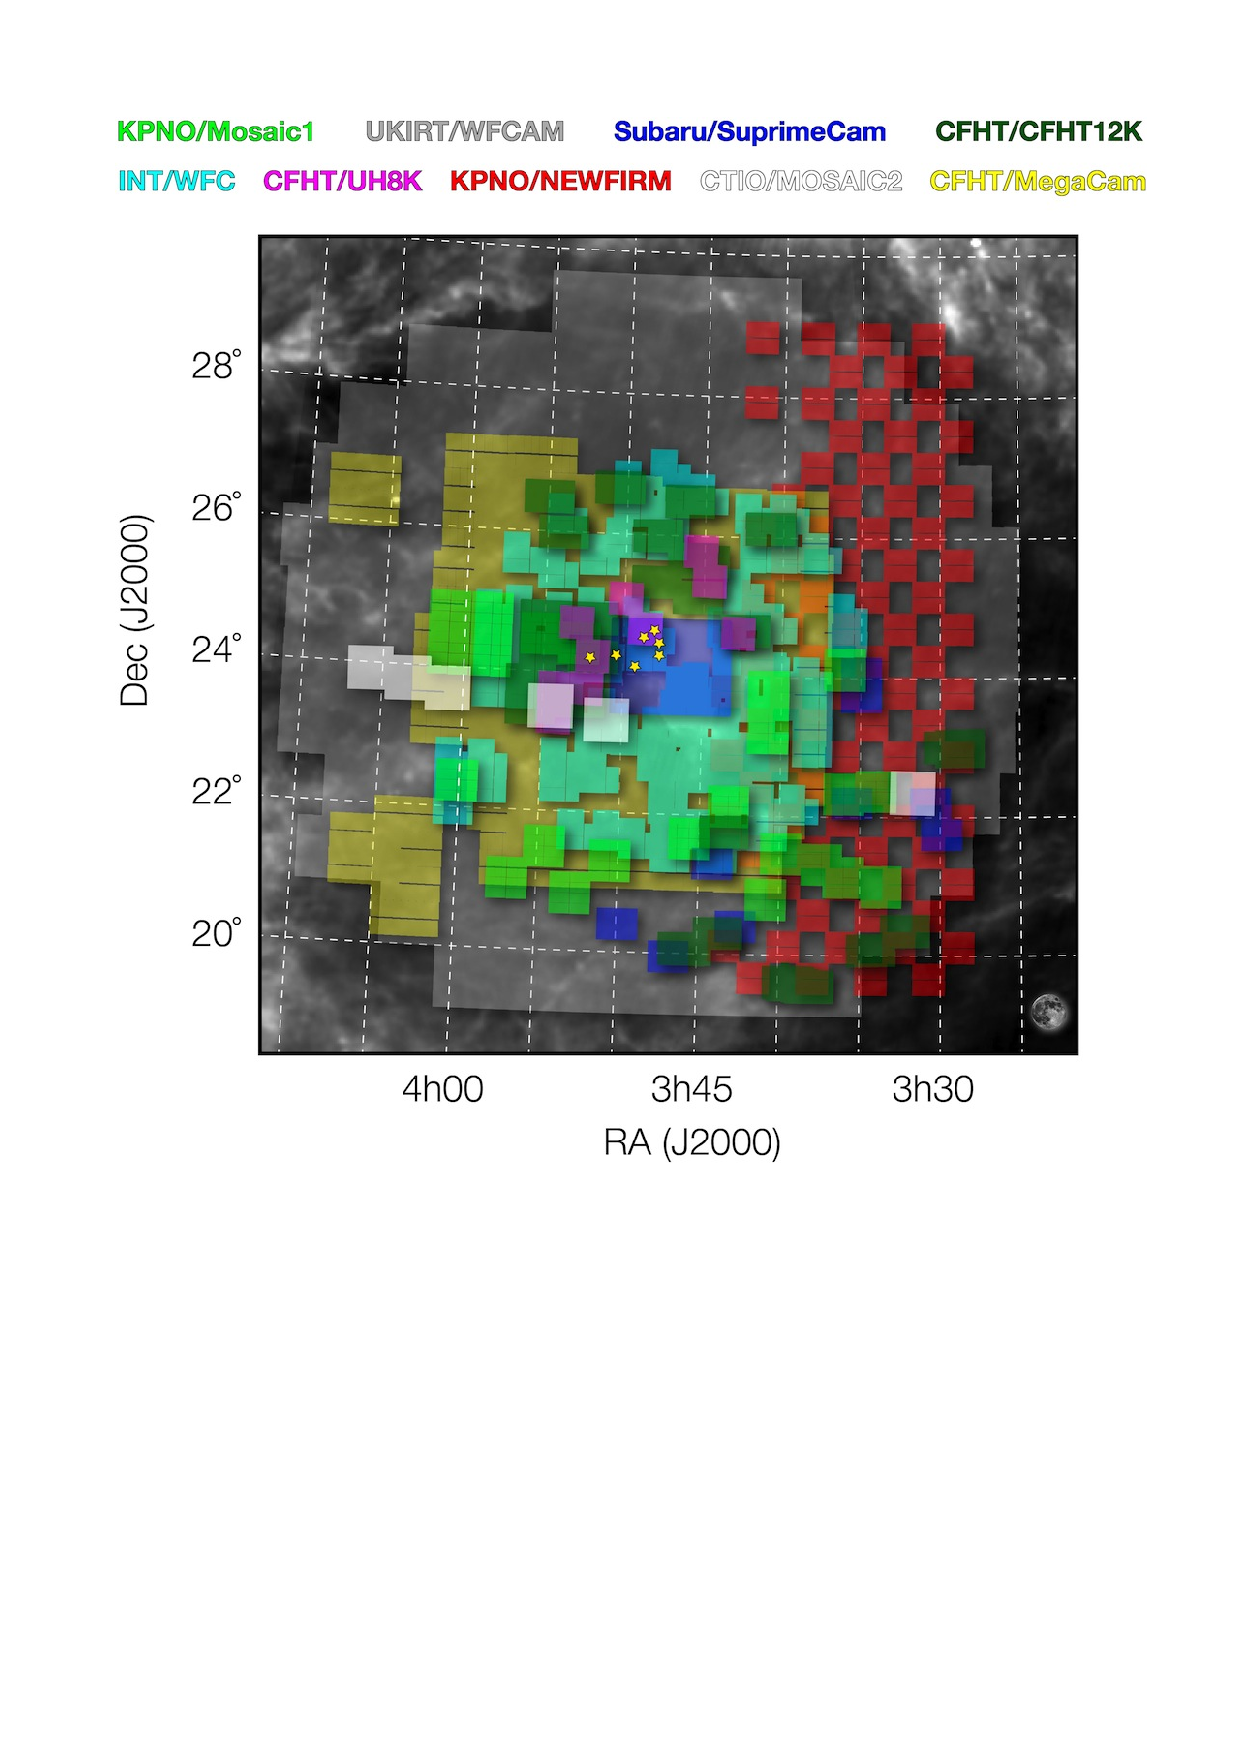
\includegraphics[width=0.7\textwidth]{../background/Figures/F1_Bouy2013.pdf}}
\only<2>{\includegraphics[width=0.7\textwidth]{Media/PM_precision.pdf}}
\only<3>{\includegraphics[width=0.7\textwidth]{Media/Pleiades-RADec2.png}}
\only<4>{\includegraphics[width=0.7\textwidth]{Media/Pleiades-Dec_i.png}}
\only<5>{\includegraphics[width=0.7\textwidth]{Media/Pleiades-Dec_K.png}}
\only<6>{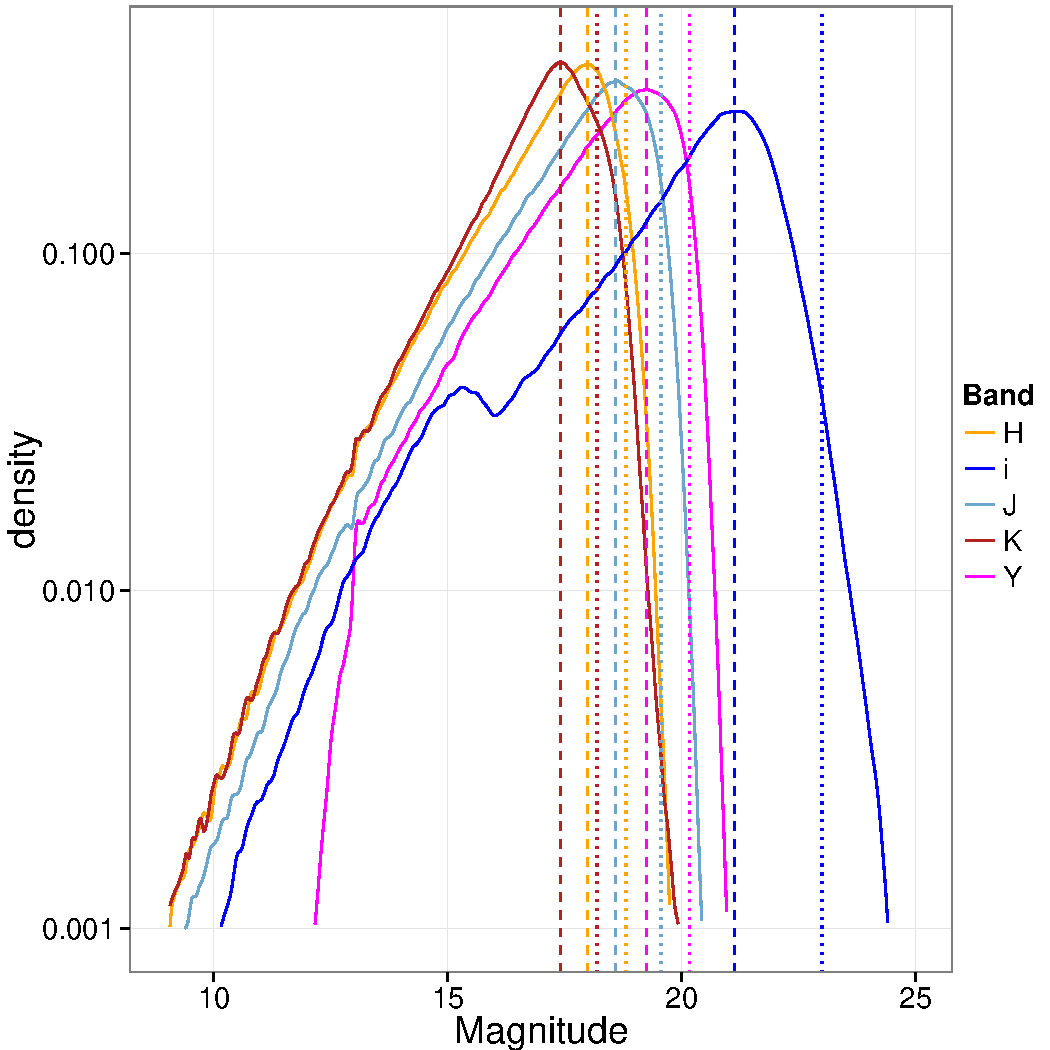
\includegraphics[width=0.6\textwidth]{../background/Figures/MagnitudeDistributionsDDR2.pdf}}
\only<7>{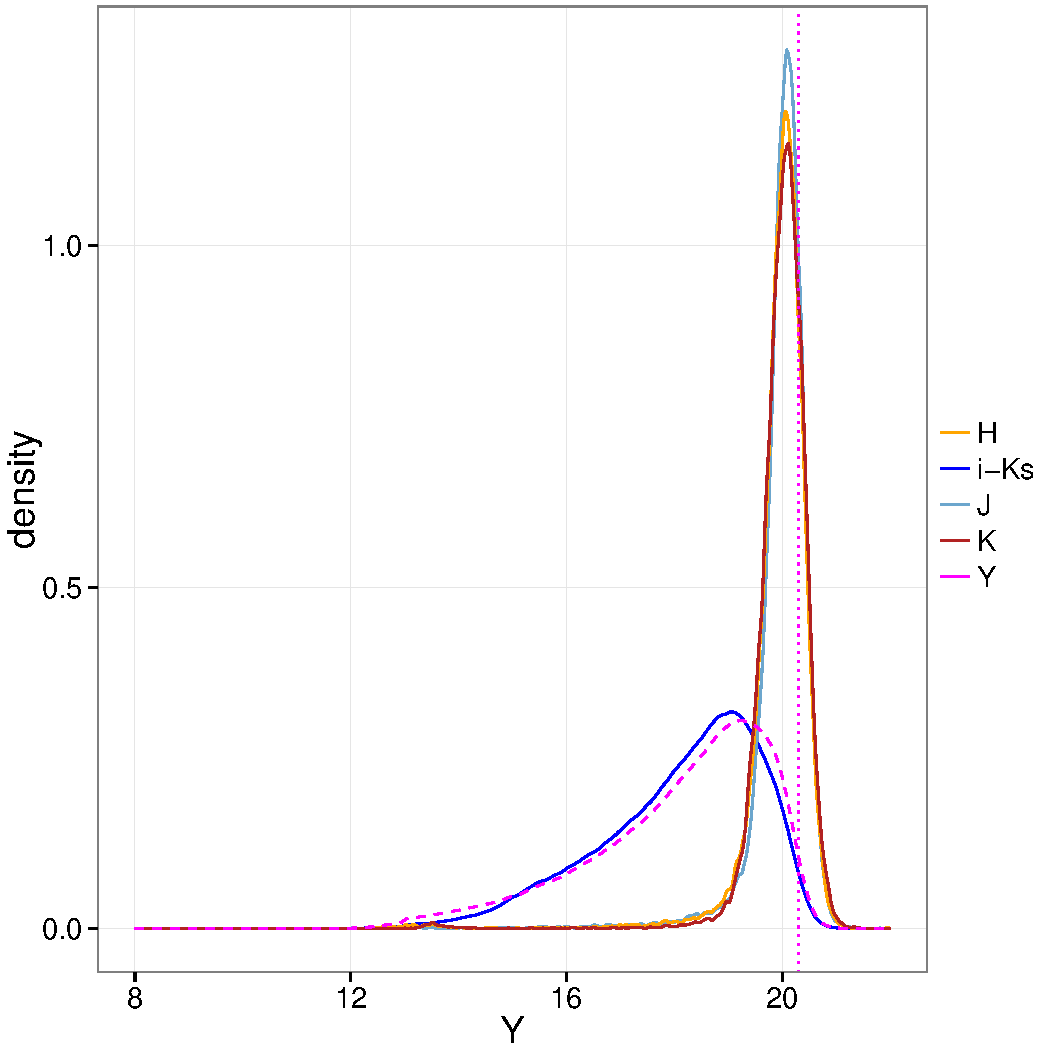
\includegraphics[width=0.6\textwidth]{../background/Figures/MissingDistributionsDDR2.pdf}}
}
\frame{
\frametitle{\hspace{2cm}RDDR2}
\begin{center}
\only<1>{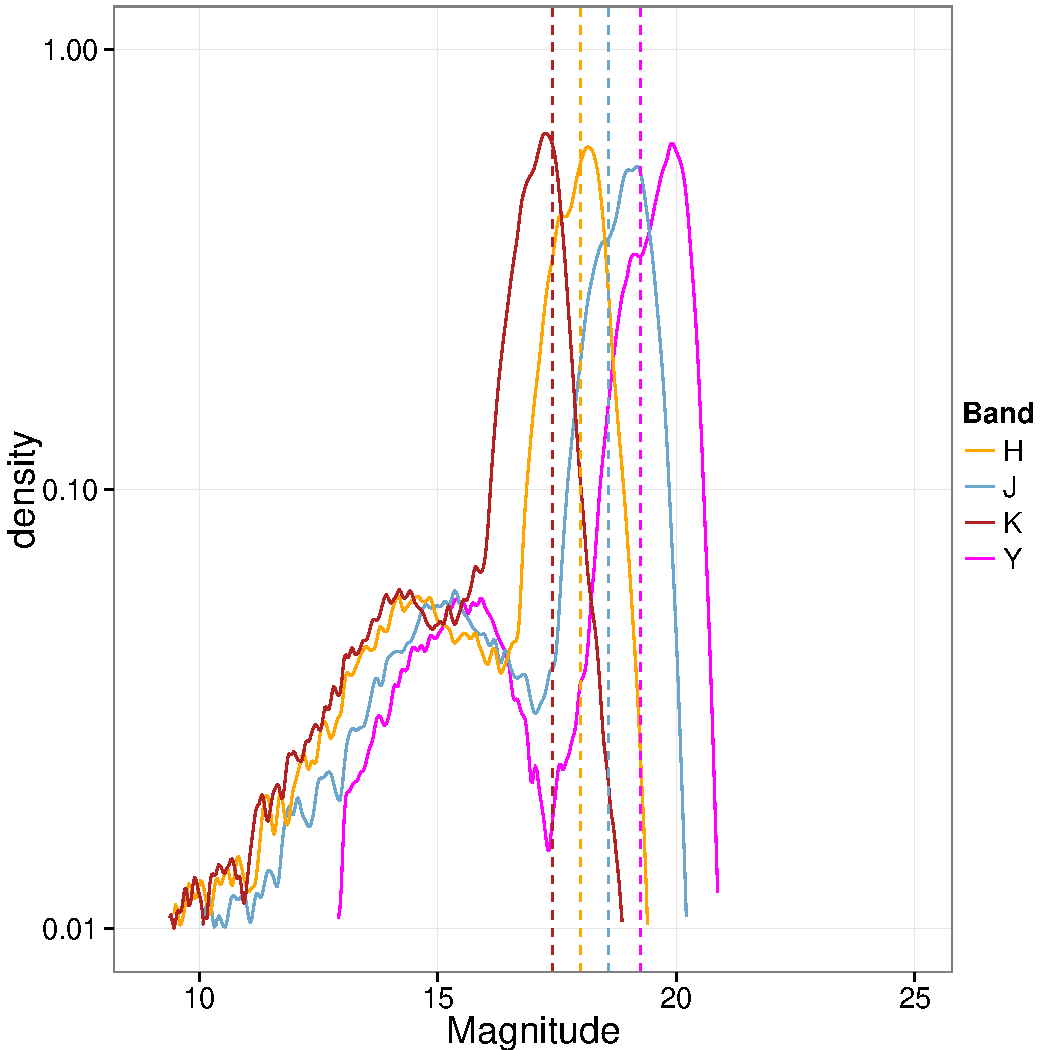
\includegraphics[page=1,width=0.6\textwidth]{../background/Figures/MagnitudeDistributions.pdf}}
\only<2>{\includegraphics[page=4,width=0.6\textwidth]{../background/Figures/MissingDistributions.pdf}}
\only<3>{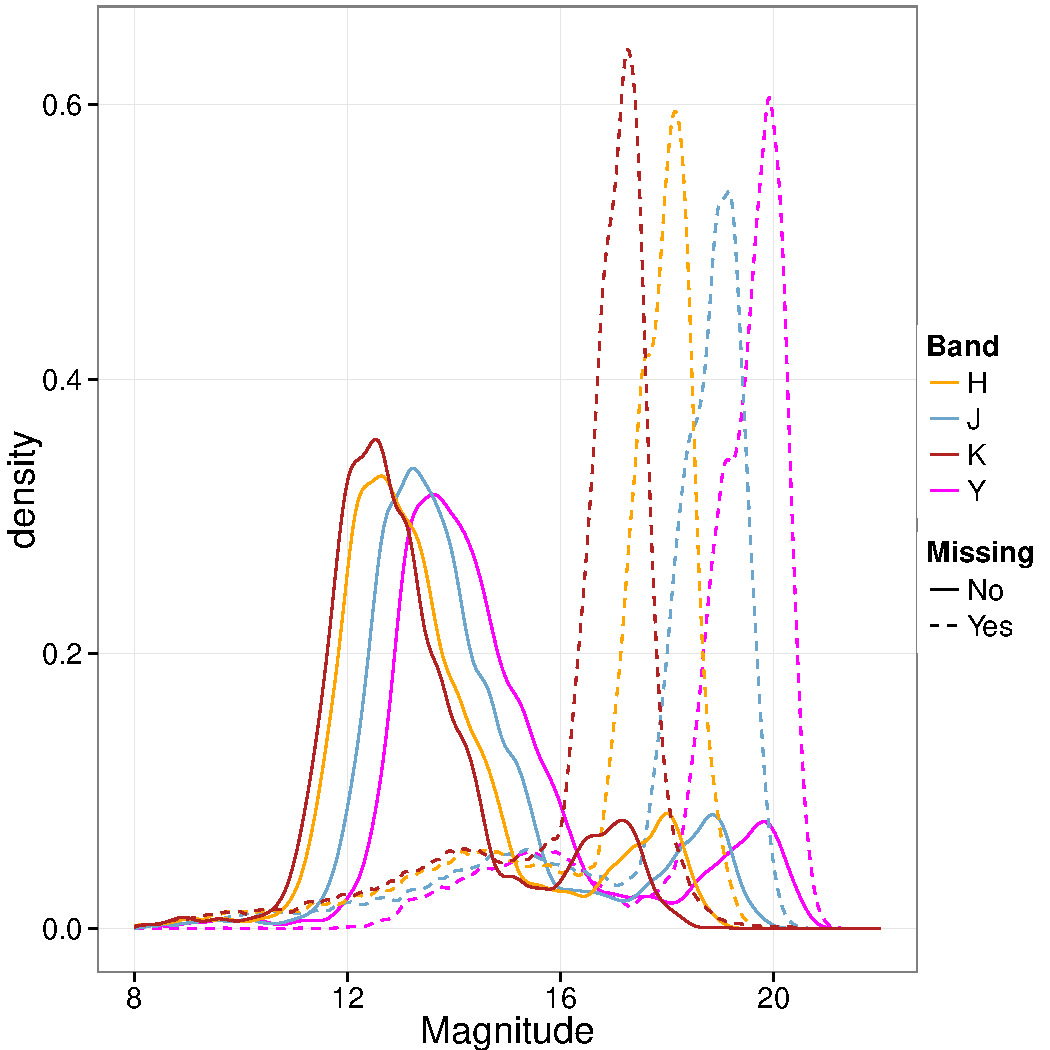
\includegraphics[width=0.6\textwidth]{../background/Figures/ObservedDistributions.pdf}}
\end{center}
\only<4>{Selection of observables:
\begin{itemize}
\item Sarro et al. 2014 -> Proper motions and $i-Ks, Y-J, J, H, K_s$
\begin{itemize}
\item Higher exhaustivity
\item Lower contamination
\item Conciseness 
\end{itemize}
\item Analysis of best models for spatial distribution
\end{itemize}
}
}
%%%%%%%%%%%%%%%%%%% METHODOLOGY %%%%%%%%%%%%%%%%%%%%%%%%%%%%
\frame{
\frametitle{\hspace{2cm}Overview of the model}

Generative model
\begin{equation}
p(\mathbf{d}_n | \pi,\boldsymbol{\theta}_c,\boldsymbol{\theta}_f,\mathbf{u}_n)=\pi \cdot p_f(\mathbf{d}_n|\boldsymbol{\theta}_f,\mathbf{u}_n) + (1-\pi)\cdot p_c(\mathbf{d}_n| \boldsymbol{\theta}_c,\mathbf{u}_n),\nonumber
\end{equation}
Membership probabilities
\begin{equation}
p( \mathcal{M}_c | \mathbf{d}_n) =\frac{p_c(\mathbf{d}_n| \boldsymbol{\theta}_c,\mathbf{u}_n)\cdot (1-\pi)}{\pi \cdot p_f(\mathbf{d}_n|\boldsymbol{\theta}_f,\mathbf{u}_n) + (1-\pi)\cdot p_c(\mathbf{d}_n| \boldsymbol{\theta}_c,\mathbf{u}_n)},\nonumber
\end{equation}
\begin{itemize}
\item Photometry independent of proper motions.
\item Cluster -> Single stars and Equal-Mass Binaries (EMB)
\end{itemize}
}
%%%%%%%%%%%%%%%%%%% Missing values %%%%%%%%%%%%%%%%%%%%%%%%%%%%
\frame{
\frametitle{\hspace{2cm}Treatment of missing information}
Types:
\begin{itemize}
\item Deterministic
\item Stochastic
\end{itemize}
Flavours:
\begin{itemize}
\item Probability of detection
\item Probability of selection
\end{itemize}
Simplistic assumptions:
\begin{itemize}
\item Field => Ignorability 
\item Cluster => Missing at random
\end{itemize}
}
%%%%%%%%%%%%%%%%%%%%%%%%%%%%%%%%%%%%%%%%%%%%%%%
\frame{
\frametitle{\hspace{2cm}Field}
\only<1>{
Model:
\begin{equation}
p_{GMM}(x|\boldsymbol{\pi},\boldsymbol{\mu},\boldsymbol{\Sigma})=\sum_{m=1}^M \pi_m \cdot \mathcal{N}(\boldsymbol{\mu}_m,\boldsymbol{\Sigma}_m),\nonumber
\end{equation}
Fitting GMMs:
\begin{itemize}
\item Proper motions => MLE
\item Photometry => MLE with missing values
\end{itemize}
}
\begin{center}
\only<2>{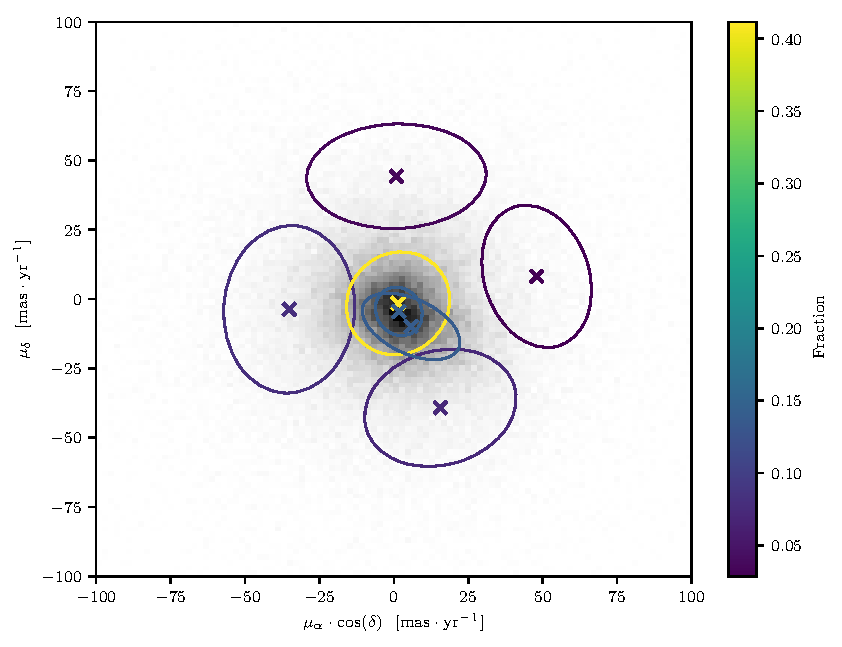
\includegraphics[page=1,width=0.7\textwidth]{../background/Figures/Field_GMM.pdf}}
\only<3>{\includegraphics[page=7,width=0.7\textwidth]{../background/Figures/Field_GMM.pdf}}
\only<4>{\includegraphics[page=5,width=0.7\textwidth]{../background/Figures/Field_GMM.pdf}}
\end{center}
}

%%%%%%%%%%%%%%%%%%%IGNORABILITY%%%%%%%%%%%%%%%%%%%%%%%%%%%%
\frame{
\frametitle{\hspace{2cm}Ignorability vs Naivety}
\begin{columns}
\begin{column}[T]{0.5\textwidth}
\includegraphics[page=4,height=0.8\textheight,width=1.2\textwidth]{../background/Figures/validationMissing.pdf}
\end{column}
\begin{column}[T]{0.3\textwidth}
\begin{itemize}
\item RMSRD density
\begin{itemize}
\item Naivety: $0.78\pm0.38$ 
\item Ignorability: $0.21\pm0.4$
\end{itemize}
\item MAR parameters
\begin{itemize}
\item Naivety: $1.5 \pm 3.2$
\item Ignorability: $0.42 \pm 2.5$
\end{itemize}
\end{itemize}
\end{column}
\end{columns}
}
%%%%%%%%%%%%%%%%%%%Cluster model%%%%%%%%%%%%%%%%%%%%%%%%%%%%
\frame{
\frametitle{\hspace{2cm}Overview}
\begin{columns}
\begin{column}[T]{0.5\textwidth}
Before:
\begin{itemize}
\item One population
\item Proper motions (1 or 2)
\item Cluster sequence
\begin{itemize}
\item Stellar models
\item PCA
\item Pincipal Curve ($\lambda$)
\end{itemize}

\end{itemize}
\end{column}
\begin{column}[T]{0.5\textwidth}
Now:
\begin{itemize}
\item Single stars and EMB
\item Proper motions (4 and 2)
\item Sequences:
\begin{itemize}
\item Empirical splines
\item Intrinsic (5D) dispersion
\item True colour distribution.
\end{itemize}
\end{itemize}
\end{column}
\end{columns}
}

%%%%%%%%%%%%%%%%%%%Cluster: PH%%%%%%%%%%%%%%%%%%%%%%%%%%%%
\frame{
\frametitle{\hspace{2cm}Cluster photometric model}
\begin{center}
\only<1>{
Colour index $i-K_s$:
\begin{enumerate}
\item Sarro et al. 2014
\item Bessel et al. 1998, $T_{eff}$  <=> M dwarfs
\item Allard et al. 2014, BT- Settl model
\end{enumerate}
}
\only<2>{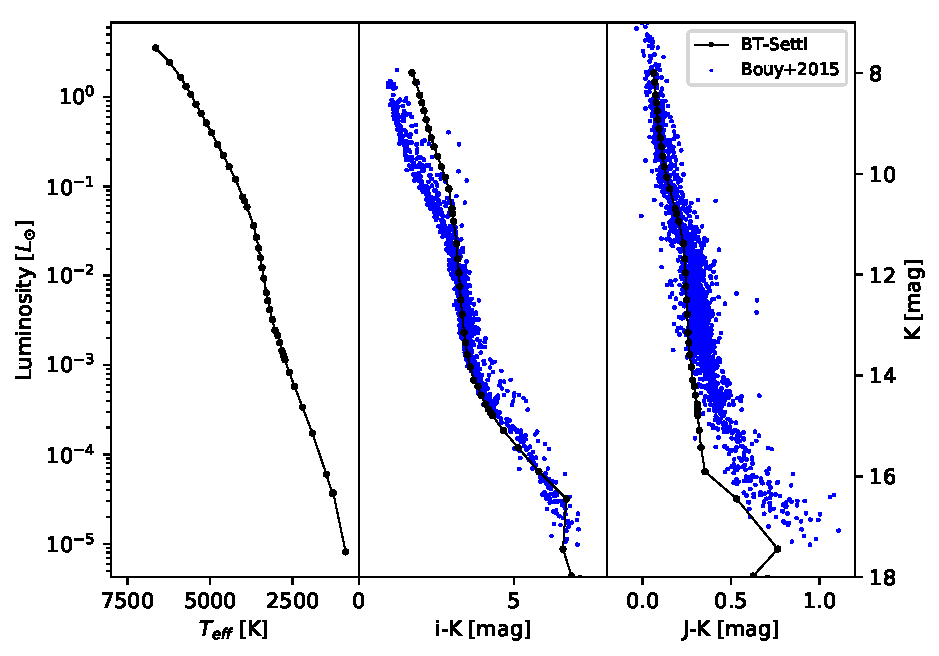
\includegraphics[page=1,width=0.7\textwidth]{../background/Figures/BT-Settl-2011bc-120Myr_Teff_vs_phot.pdf}}
\only<3>{\includegraphics[page=3,width=0.7\textwidth]{../background/Figures/BT-Settl-2011bc-120Myr_Teff_vs_phot.pdf}}
\only<4>{\includegraphics[page=7,width=0.6\textwidth]{../background/Figures/Photometry_fit.pdf}}
\only<5>{\includegraphics[page=8,width=0.6\textwidth]{../background/Figures/Photometry_fit.pdf}}
\only<6>{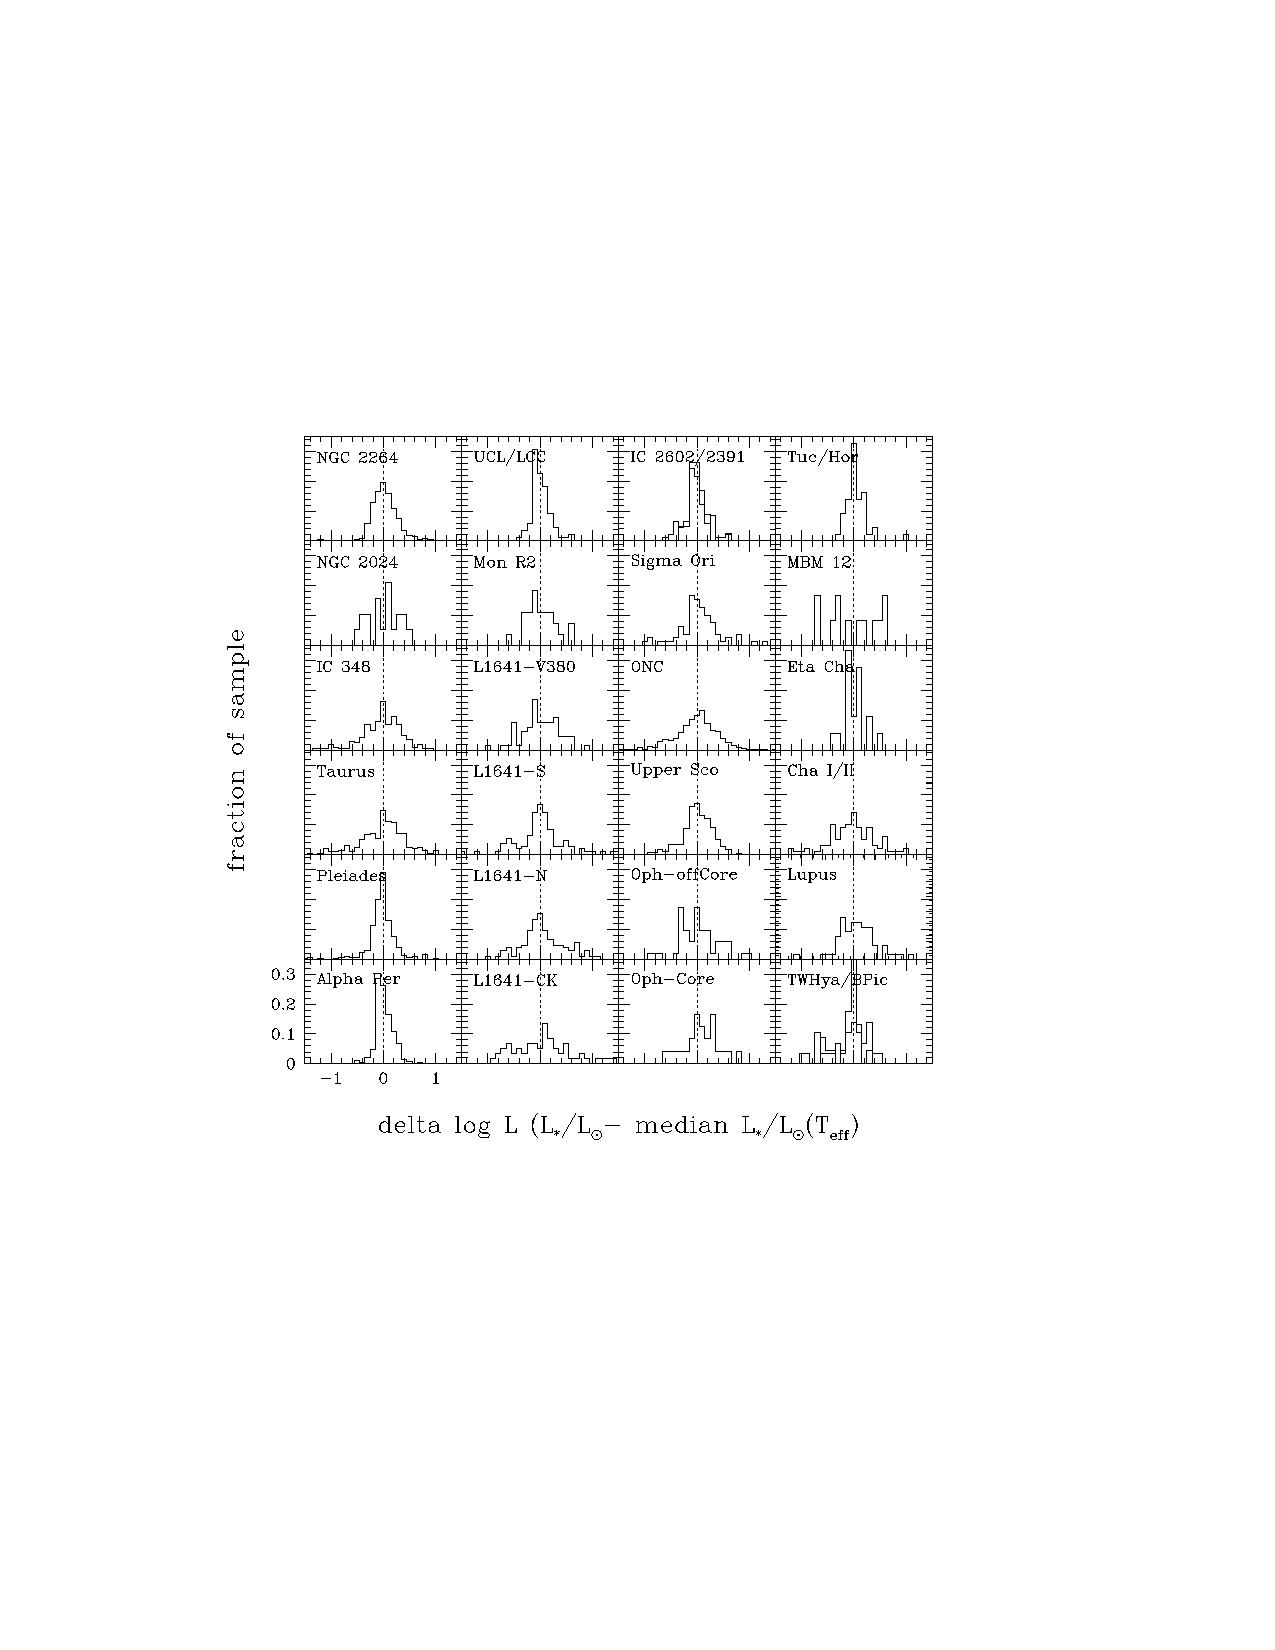
\includegraphics[width=0.6\textwidth]{../background/Figures/F2_Hillenbrand2008.pdf}}
\end{center}
}

%%%%%%%%%%%%%% RESULTS on SYNTHETIC DATA%%%%%%%%%%%%%%%%%%%%%%%%%%%%%%%%%
\frame{
\frametitle{\hspace{2cm}Validation on synthetic data}
\only<1>{
Five synthetic data sets: with and without missing values.
\begin{align}
TPR &= \frac{TP}{TP+FN} \nonumber \\
FPR &= \frac{FP}{FP+TN} \nonumber \\
CR   &= \frac{FP}{FP+TP} \nonumber \\
PPV &= \frac{TP}{TP+FP} \nonumber \\
ACC &= \frac{TP+TN}{TN+FN+TP+FP},\nonumber
\end{align}}
\begin{center}
\only<2>{
$\langle CR \rangle=5.8\pm 0.2$\% \\ 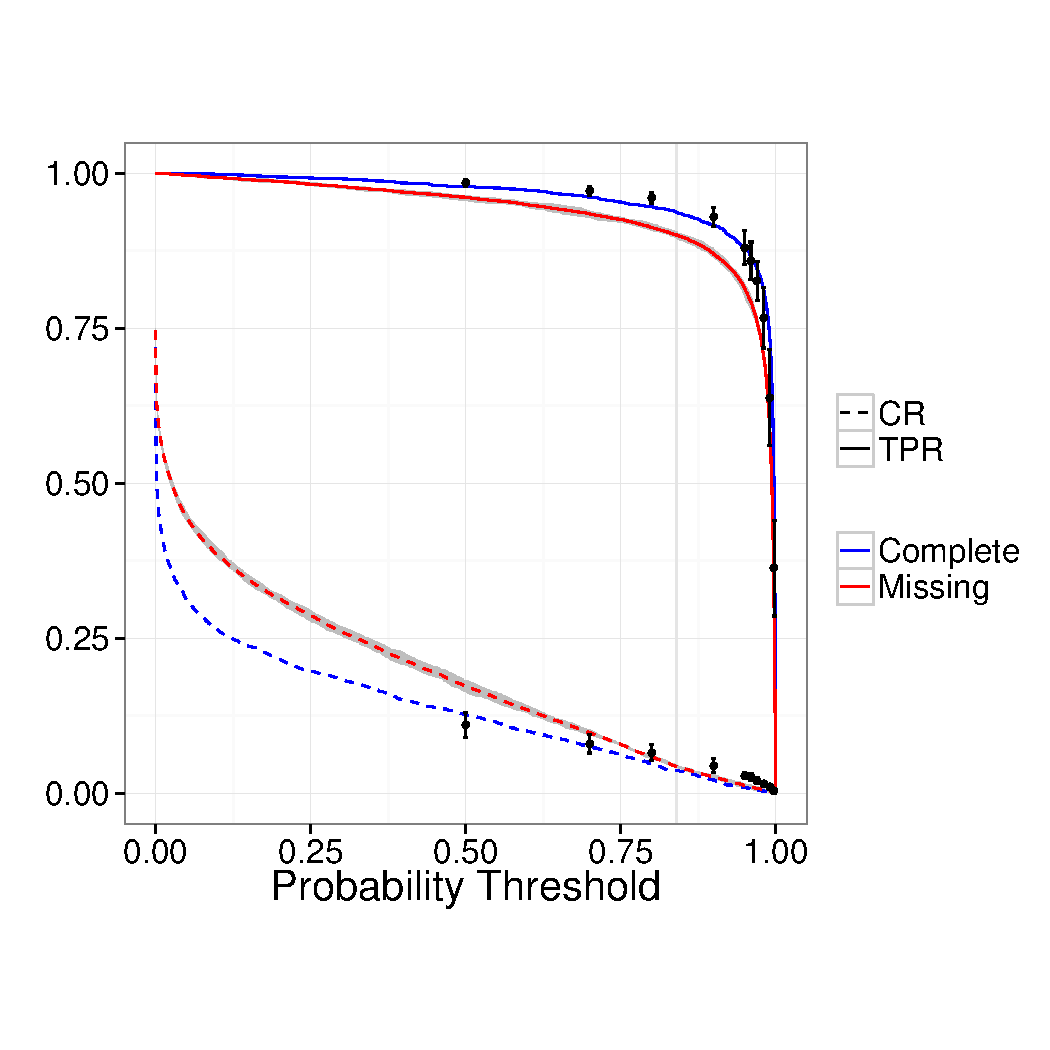
\includegraphics[page=1,width=0.7\textwidth]{../background/Figures/FTPRvsSarro.pdf}}
\only<3>{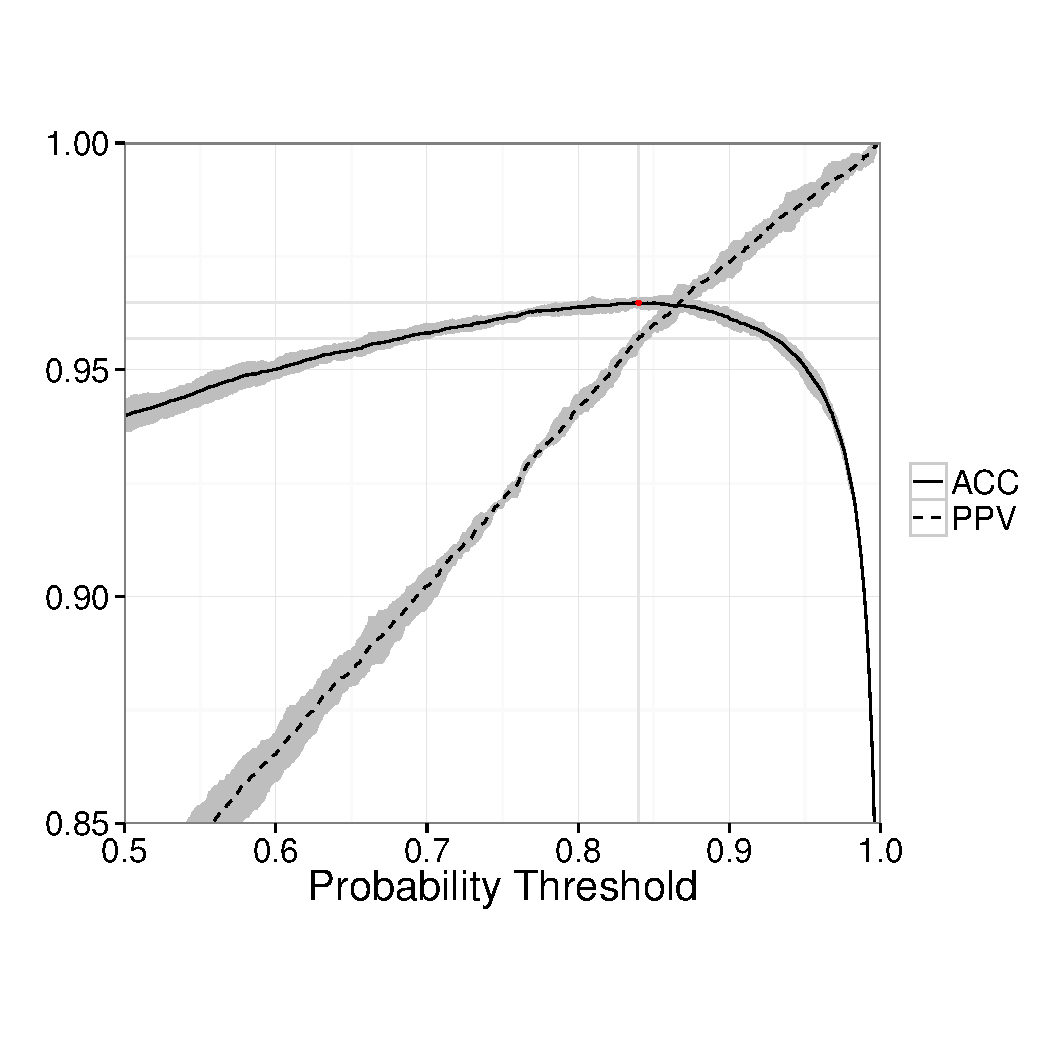
\includegraphics[page=1,width=0.5\textwidth]{../background/Figures/PrecisionAccuracy.pdf}\\
 ACC=$96.5\pm0.1$\%, CR=$4.3\pm0.2$\%, TPR=$90.0\pm0.05$\%, PPV=$95.6\pm0.2$\%. }
\end{center}
}
%%%%%%%%%%%%%%%%%%%%Comparison with literature%%%%%%%%%%%%%%%%%%%%%%%%%
\frame{
\frametitle{\hspace{2cm}Comparison with literature}
\begin{center}
\only<1>{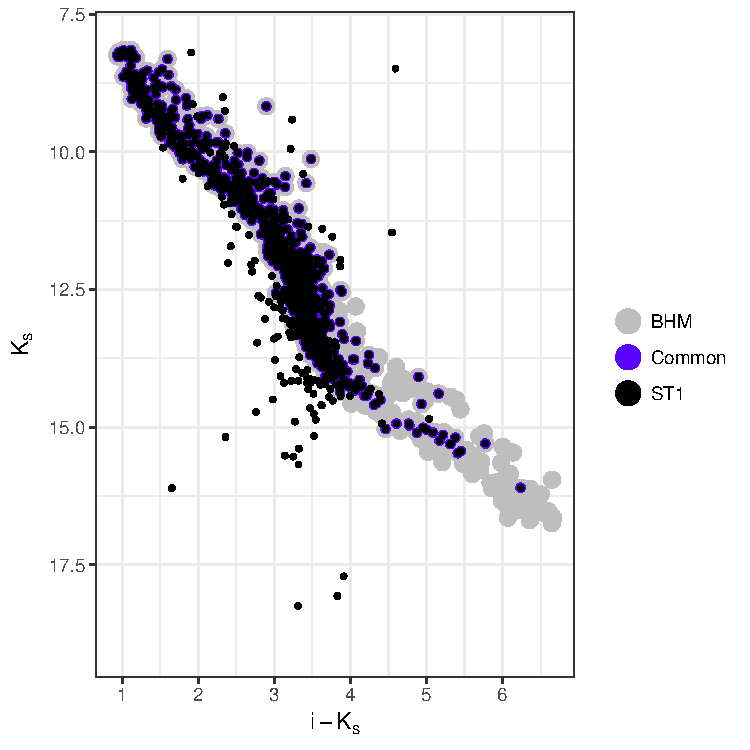
\includegraphics[page=1,width=0.6\textwidth]{../background/Figures/ST1_ph-eps-converted-to.pdf}}
\only<2>{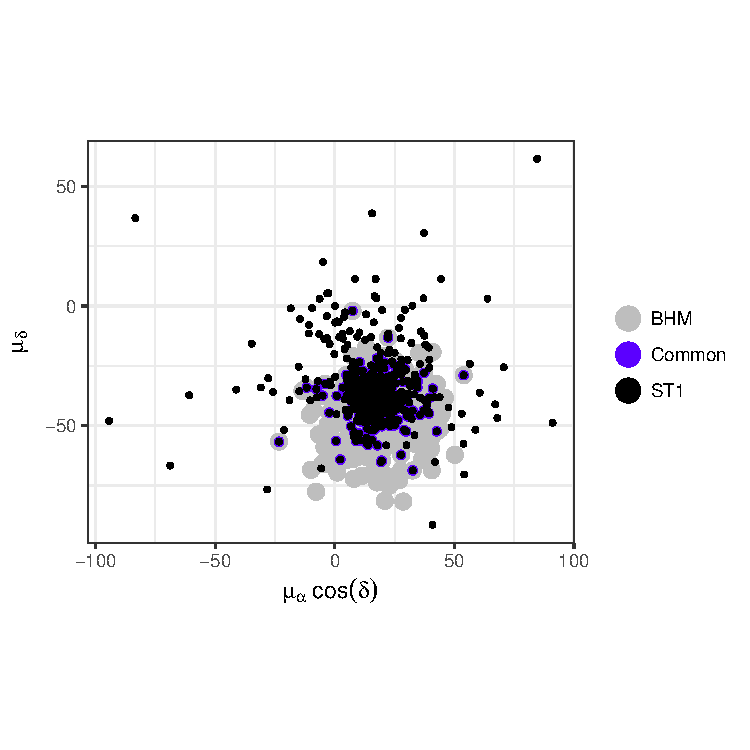
\includegraphics[page=1,width=0.6\textwidth]{../background/Figures/ST1_pm-eps-converted-to.pdf}}
\only<3>{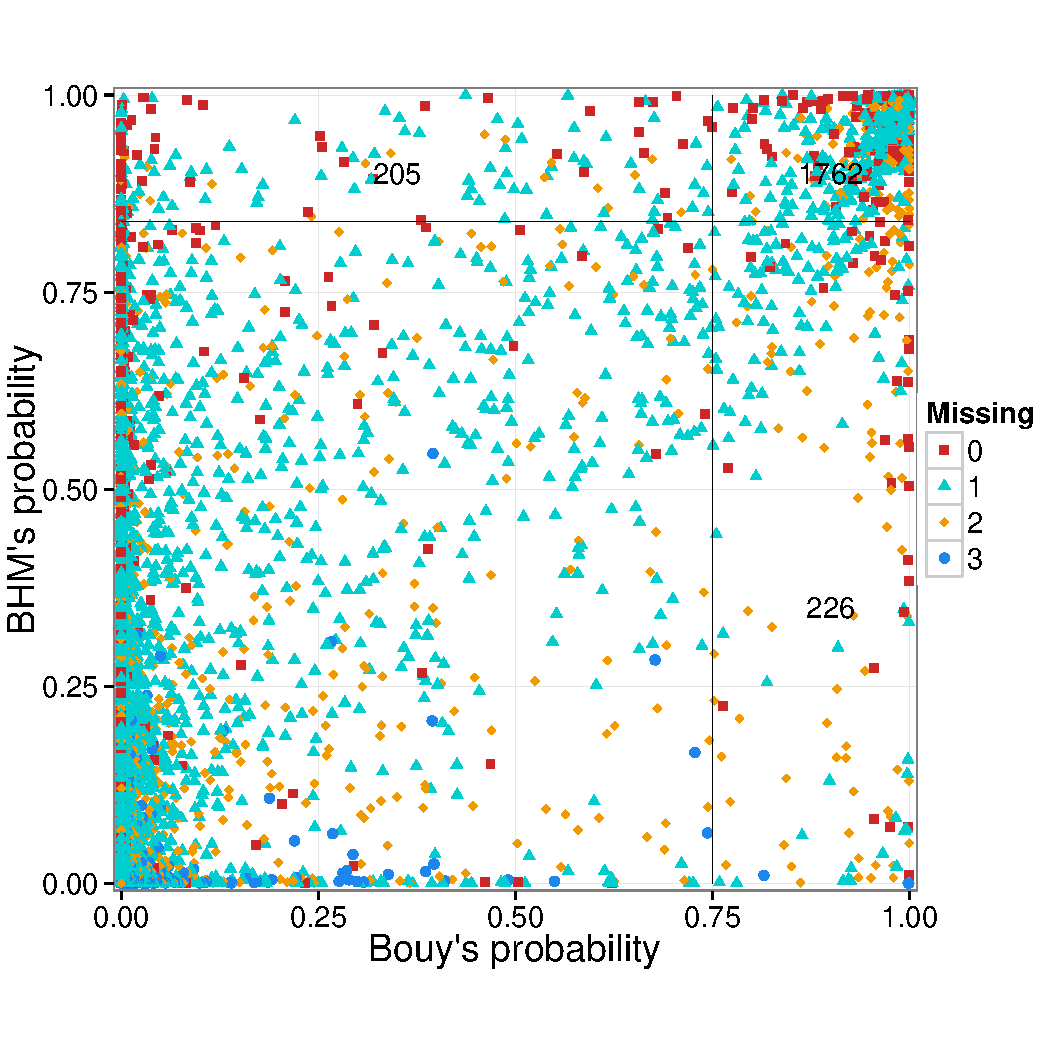
\includegraphics[page=1,width=0.6\textwidth]{../background/Figures/BHM/BHMvsBouy.pdf}}
\only<4>{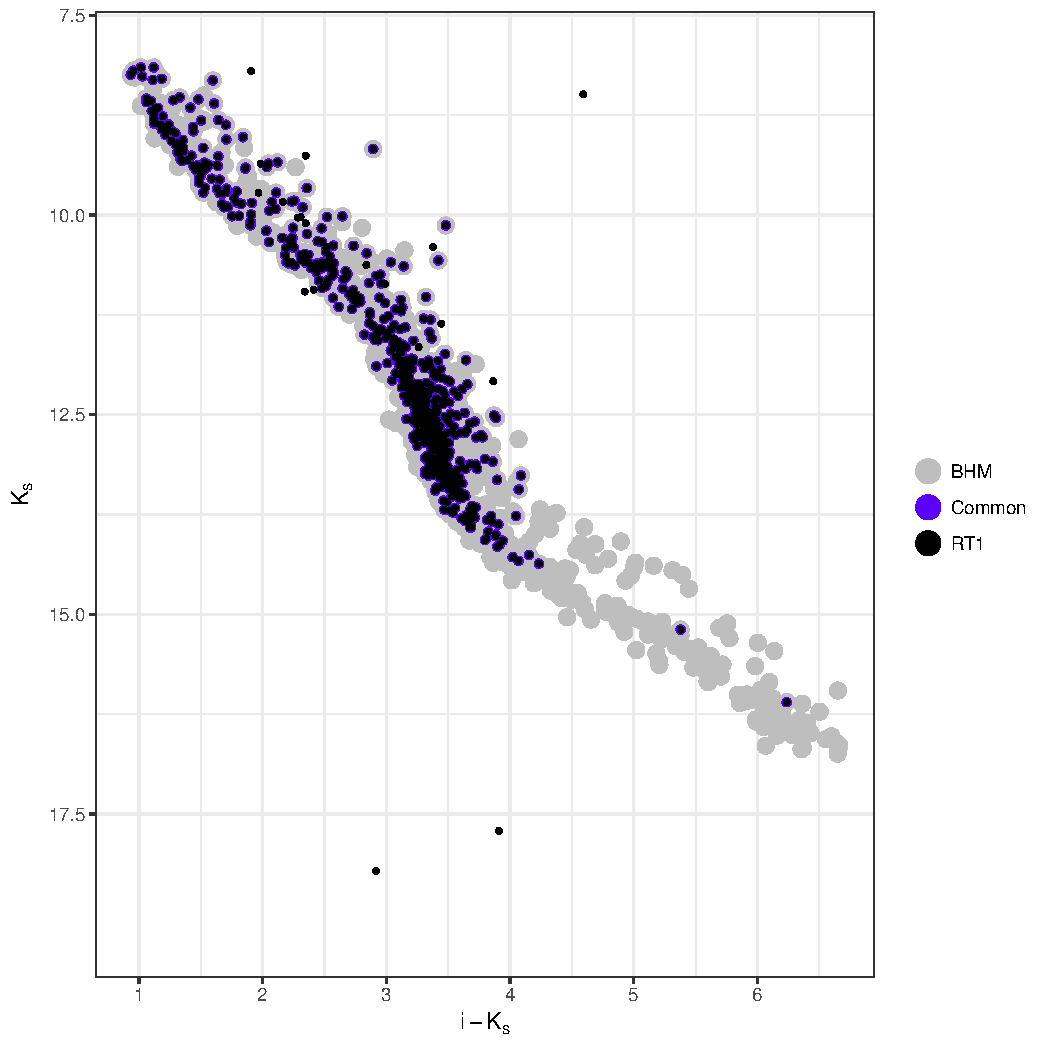
\includegraphics[page=1,width=0.6\textwidth]{../background/Figures/RT1_ph-eps-converted-to.pdf}}
\only<5>{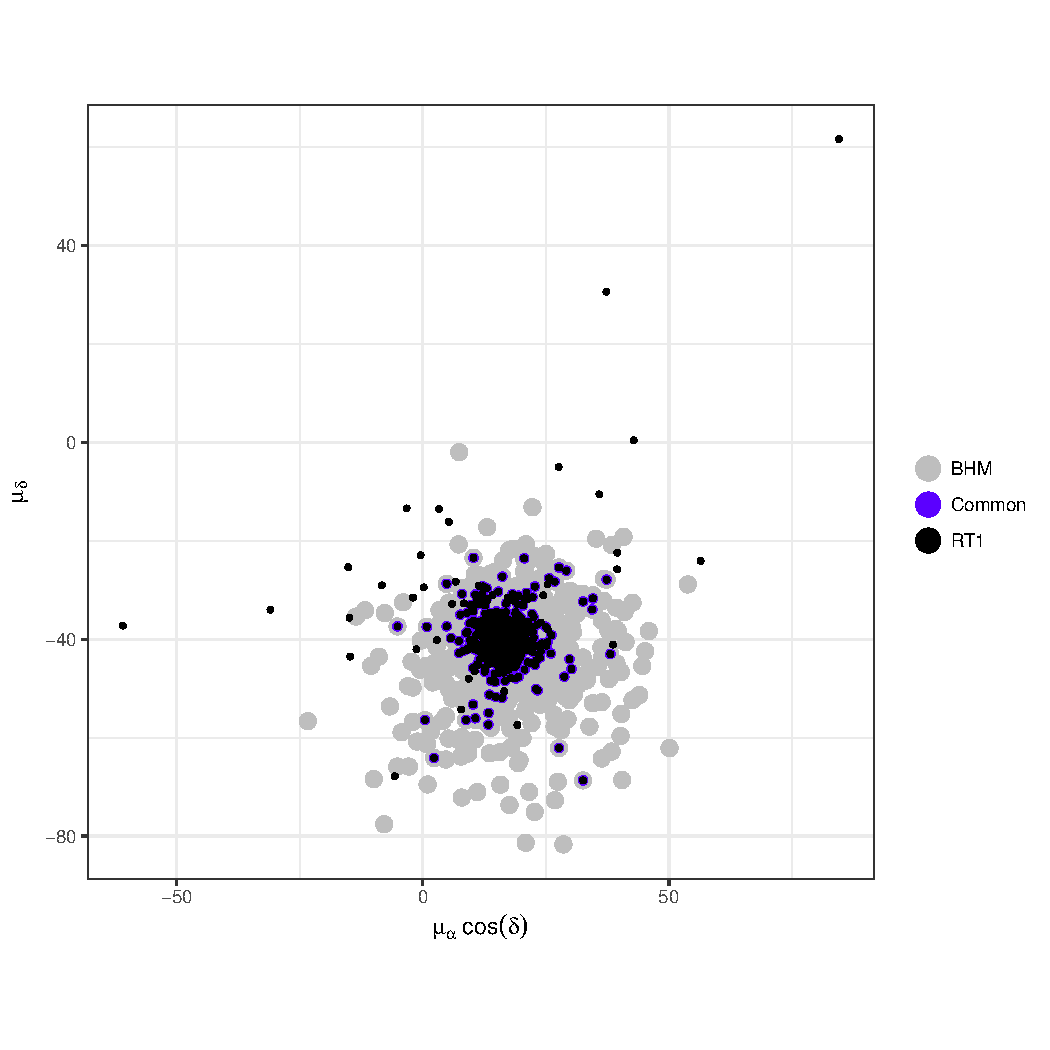
\includegraphics[page=1,width=0.6\textwidth]{../background/Figures/RT1_pm-eps-converted-to.pdf}}
\end{center}
}
%%%%%%%%%%%%%%%%%%%%%% RESULTS%%%%%%%%%%%%%
\frame{
\frametitle{\hspace{2cm}Results}
\begin{center}
\only<1>{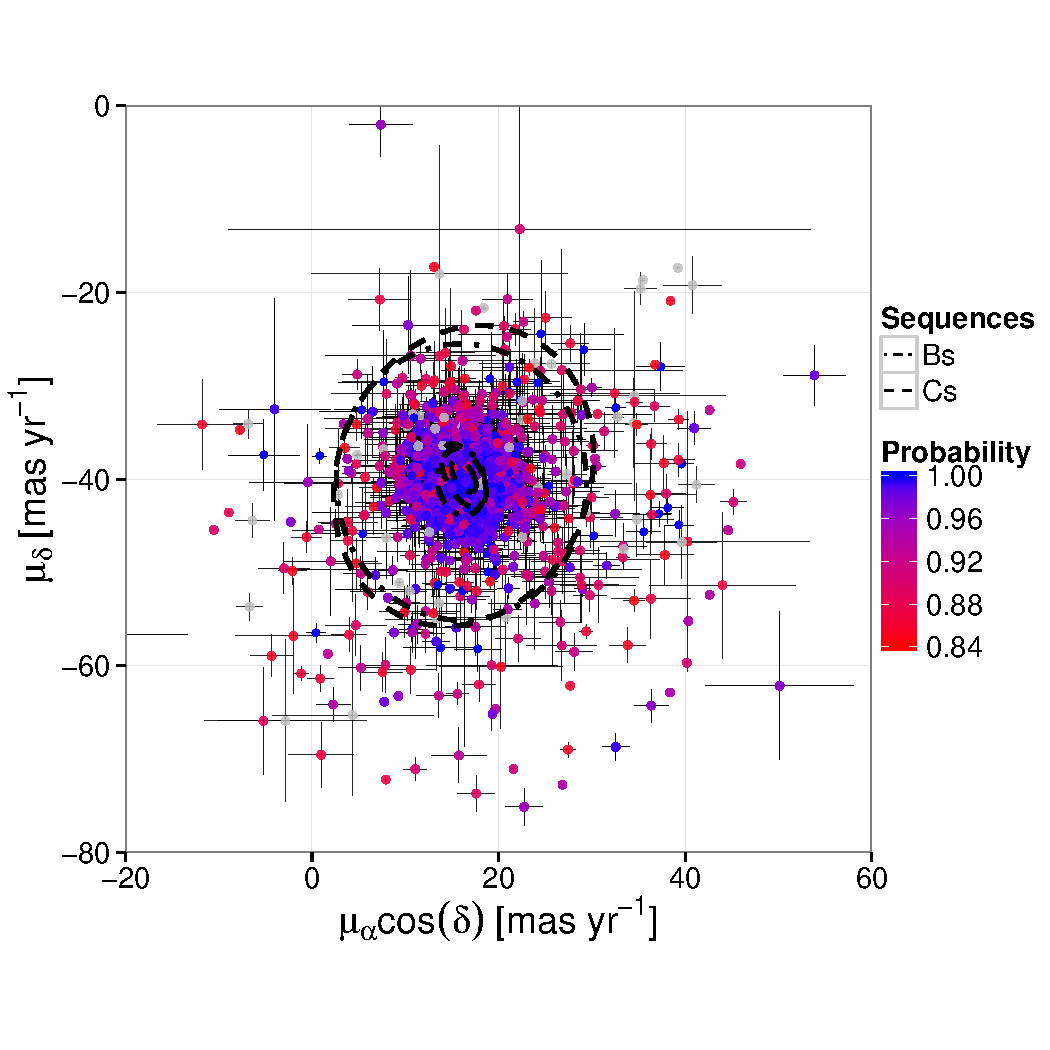
\includegraphics[page=1,width=0.7\textwidth]{../background/Figures/BHM/Probability.pdf}}
\only<2>{\includegraphics[page=5,width=0.6\textwidth]{../background/Figures/BHM/Probability.pdf}}
\only<3>{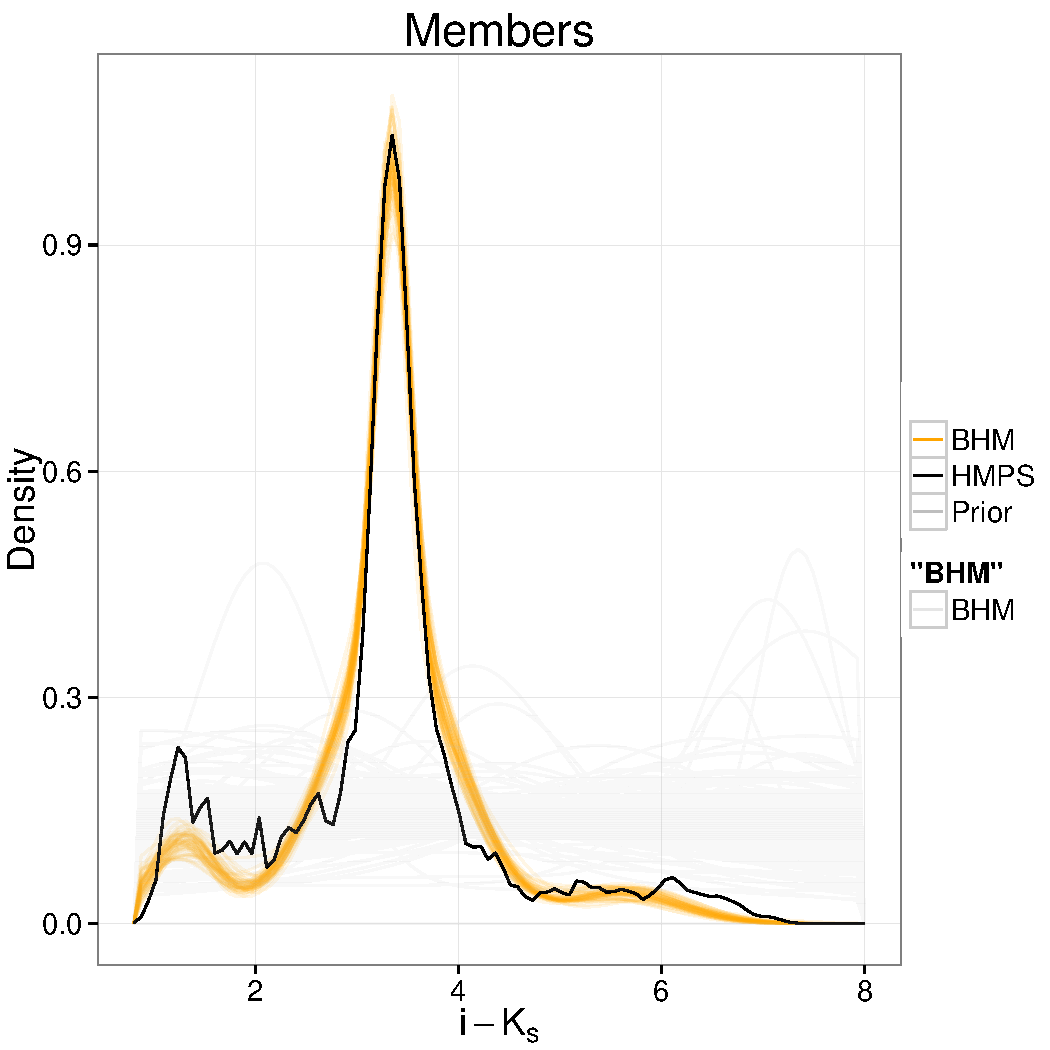
\includegraphics[page=1,width=0.6\textwidth]{../background/Figures/BHM/MembersModel.pdf}}
\only<4>{\includegraphics[page=2,width=0.6\textwidth]{../background/Figures/BHM/MembersModel.pdf}}
\only<5>{\includegraphics[page=10,width=0.6\textwidth]{../background/Figures/BHM/MembersModel.pdf}}
\only<6>{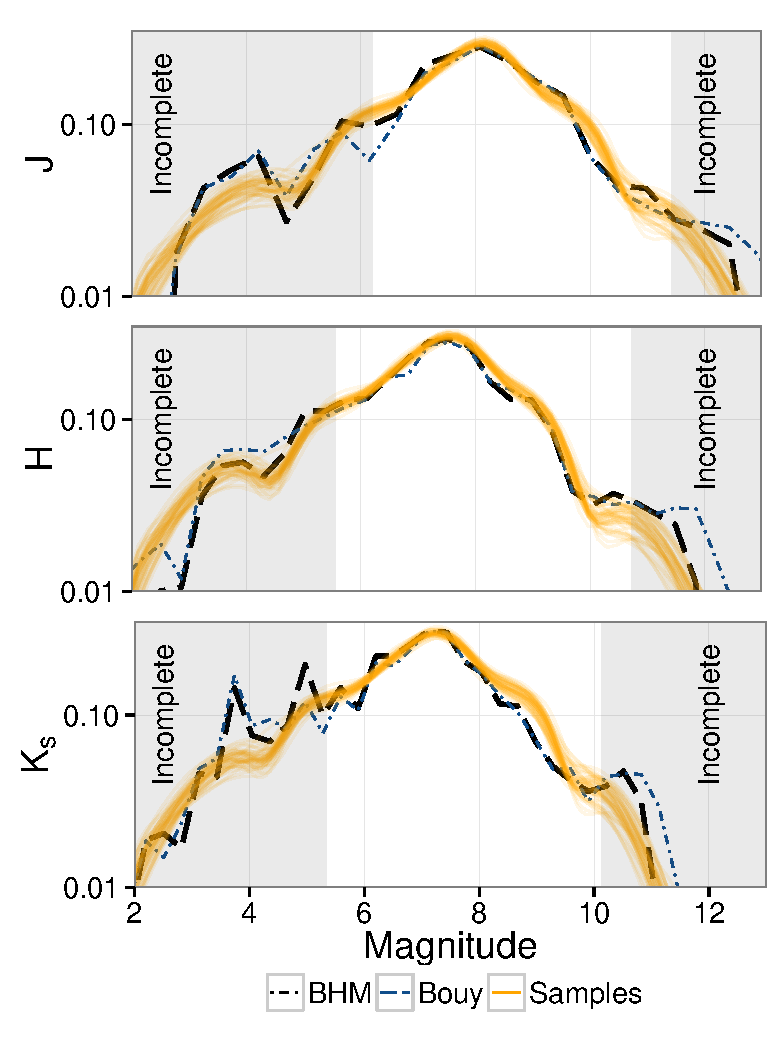
\includegraphics[page=1,width=0.5\textwidth]{../background/Figures/BHM/absolute_JHK-log.pdf}}
\only<7>{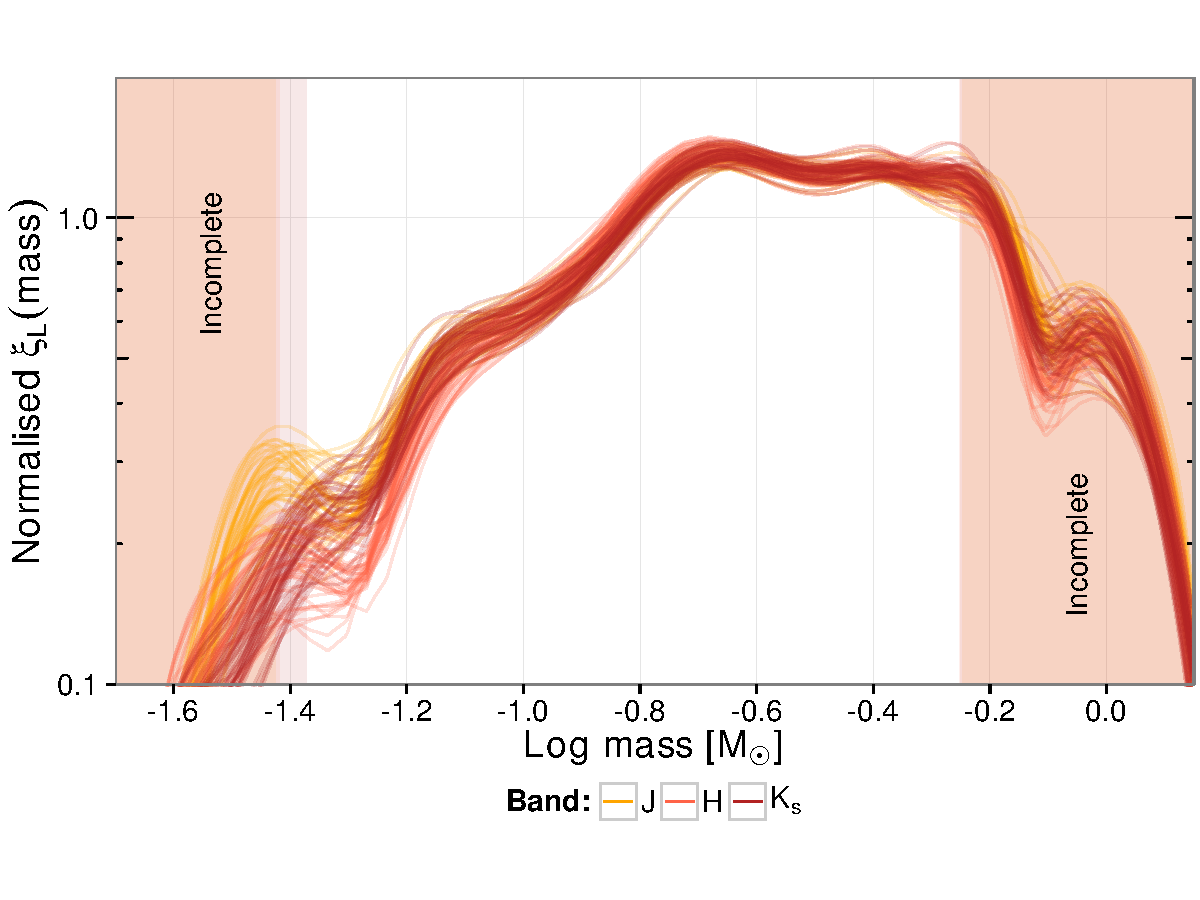
\includegraphics[page=1,width=0.6\textwidth]{../background/Figures/BHM/MassDistribution.pdf}}
\only<8>{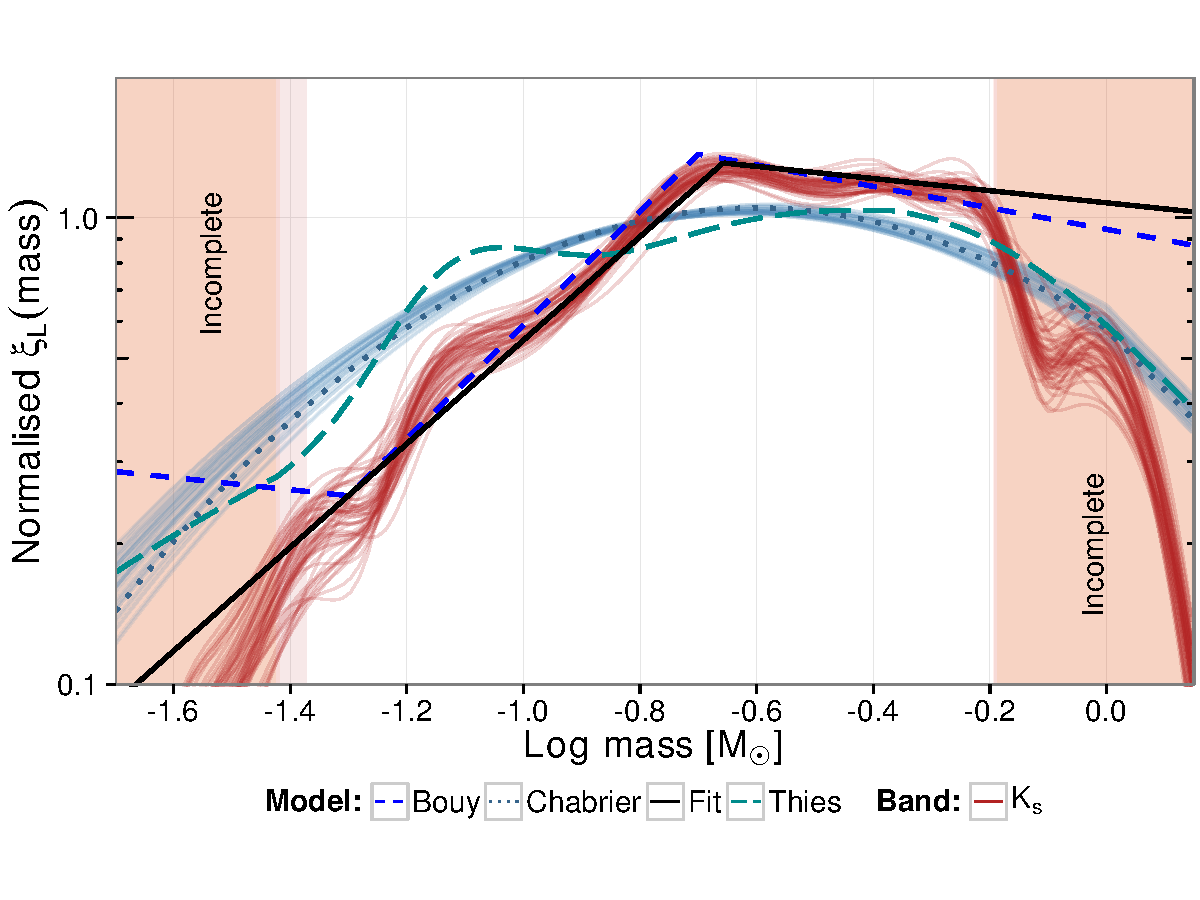
\includegraphics[page=1,width=0.6\textwidth]{../background/Figures/BHM/ModelsMassDistribution.pdf}}
\end{center}
}
\frame{
\frametitle{\hspace{2cm}Conclusions}
\begin{itemize}
\item Accurate statistical distributions
\item Membership probabilities for $10^5$ objects
\item 205 new members
\item Mass distribution with uncertainties from all observables.
\end{itemize}
}

\end{document}
